%        File: apache.tex
%     Created: sáb ene 16 06:00  2016 C
% Last Change: sáb ene 16 06:00  2016 C
%
\documentclass[a4paper, 11pt]{article}
\usepackage[utf8]{inputenc}
\usepackage[catalan]{babel}
\usepackage[obeyspaces]{url}
\usepackage{comment}
\usepackage{hyperref}
\usepackage[pdftex]{graphicx}
%\setlength{\parindent}{5pt}
\begin{document}
\title{Apunts d'Apache}
\author{Juan Aguilera}
\maketitle

\begin{comment}
oddsidemargin \the\oddsidemargin \newline
textwidth \the\textwidth \newline
marginparsep \the\marginparsep \newline
marginparwidth \the\marginparwidth \newline
hoffset \the\hoffset \newline
paperwidth \the\paperwidth 
\end{comment}

\section{Instal·laci\'o del paquet apache}
\paragraph{Versió d'apache \\}

\scalebox{.5}{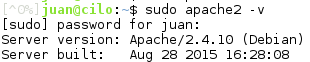
\includegraphics{apache_version.png}}

d'entre les novetats de la versió apache 2.4 respecte les versions anteriors cap destacar que la directiva \textit{NameVirtualHost} ja no \'es útil i \'es \textit{deprecated}.

Una altra novetat \'es que es poden definir variables en la configuració.

Per m\'es info, veure \href{https://httpd.apache.org/docs/2.4/new_features_2_4.html}{les new features d'apache a la pàgina oficial}\cite{DOC}.

\section{Configuració d'apache}
\subsection{fitxer de configuració principal}
\paragraph{jugant amb l'index.html }
Traient l'index.html de /var/www podem veure els directoris que es troben a www. Això s perque deu haver-hi per defecte un “DirectoryIndex index.html” i un “Option Indexes” si esborres el fitxer es mostra tot. Això \'es degut a que en apache2.conf ho han definides tres directives \textit{Directory} per configurar com s'ha de comportar el servei quan s'intenta accedir a aquesta ruta:

\scalebox{.6}{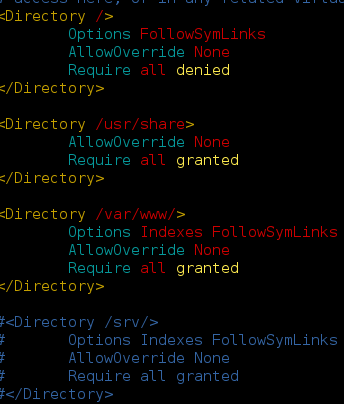
\includegraphics{index_html.png}}

\subsection{fitxer de configuració de ports}
És on especifiquem els ports on ha d'escoltar el dimoni.
\section{Principals directives}

Tota la documentació sobre qualsevol directiva es pot trobar \href{https://httpd.apache.org/docs/2.4/mod/directives.html}{en la pàgina de referència de directives d'apache}

Per entendre les directives a apache \'es important saber en quins contextos es poden utilitzar. Hi han els següents:

\subsection{\href{http://localhost/apache2-doc/es/mod/directive-dict.html#Context}{Context}} Indica en quin àmbit o àmbits s'aplica la directiva:
\paragraph{server config} This means that the directive may be used in the server configuration files (e.g., apache2.conf), but not within any \verb+<VirtualHost>+ or \verb+<Directory>+ containers. It is not allowed in .htaccess files at all. 
\paragraph{virtual host} This context means that the directive may appear inside \verb+<VirtualHost>+ containers in the server configuration files. 
\paragraph{directory} A directive marked as being valid in this context may be used inside \verb+<Directory>+, \verb+<Location>+, \verb+<Files>+, and \verb+<Proxy>+ containers in the server configuration files, subject to the restrictions outlined in Configuration Sections. 
\paragraph{.htaccess} If a directive is valid in this context, it means that it can appear inside per-directory .htaccess files. It may not be processed, though depending upon the overrides currently active. 
\subsection{Taula de directives}
\begin{tabular}{|p{4cm}|p{3cm}|p{5cm}|}
\hline
\textbf{Directiva} & \textbf{Context} & \textbf{Descripció} \\
\hline
AllowOverride & directory & Què directives es poden posar en el fitxer \textit{.htacces}. Per defecte el seu valor \'es none.\\
\hline
DirectoryIndex & server config, virtual host, directory, .htaccess & Diu què mostrar quan l'usuari demana una URL que fa referència a un directori i acabant amb una \slash\\
\hline
Options & server config, virtual host, directory, .htaccess & Configura qu\'e característica està disponible en un directory en un àmbit en particular.\\
\hline
NameVirtualHost & & \textbf{DEPRECATED en apache 2.4}\\
\hline
DocumentRoot & Server config; VirtualHost& Les adreces demanades pel client seràn relatives a aquesta ruta. Httpd servirà fitxers relatius a la ruta.\\
\hline
ServerRoot & server config& indica el directoi base per la configuració d'apache.\\
\hline
ServerName & server config; Virtualhost& Nom de servidor i port que el servei utilitza per identificar-se a si mateix.\\
\hline
ServerAlias & Virtualhost& Alias per el nom del servidor.\\
\hline
VirtualHost & server config & context per configurar un virtualhost.\\
\hline
Directory & server config; VirtualHost& Enclose a group of directives that apply only to the named file-system directory, sub-directories, and their contents\\
\hline
Location & server config; VirtualHost& Applies the enclosed directives only to matching URLs.\\
\hline
Files & server config; VirtualHost; Directory; .htaccess& Contains directives that apply to matched filenames. 
Exemple: 
\footnotesize{\verb+<Files ~ ``\.(gif|png)$''>+}.\\
\hline
\end{tabular}

\begin{tabular}{|p{4cm}|p{3cm}|p{5cm}|}
\hline
\textbf{Directiva} & \textbf{Context} & \textbf{Descripció} \\
\hline
Allow, Deny, Order & Directory; .htaccess& \textbf{DEPRECATED}. Substituit pels \textit{Require}, \textit{RequireAny|All|None} \\
\hline
RequireAll & Directory; .htaccess & totes les directives Require dintre d'aquesta s'han de complir. \\
\hline
RequireAny & Directory; .htaccess & Alguna de les directives \textit{Require} dintre d'aquesta s'han de complir. Si hi han directives \textit{Require} que no estan dintre de les \textit{Require*} aleshores s'interpreten com a que es troben en el \textit{RequireAny}\\
\hline
\end{tabular}

\paragraph{Options}
Pot ser \textit{None} o m\'es d'entre molts valors d'entre els que destaquen:

\begin{itemize}
	\item \textit{FollowSymlinks}: Es permeten les peticions a enllaços simbòlics que hi hagin en el directori.
	\item \textit{Indexes}: Si demanem una URL corresponent a un directori, mostra el que haguem escollit amb la directiva \textit{DirectoryIndex} (en cas que no hi hagi DirectoryIndex).
	\item \textit{All}: Tots.
\end{itemize}

\textbf{Nota:} Amb els signes \textit{+} o \textit{-} davant dels diferents valors que pot prendre \textit{Opions} voldrà dir que afegim o traiem llurs valors (si n'hi ha algun amb signe o han d'estar tots).

\paragraph{DirectoryIndex}

Lista de recursos que el cliente puede encontrar en un directorio dado cuando el cliente solicita la URL de ese directorio acabada en \slash. En la lista podemos poner ficheros que estan en el directorio o rutas relativas que estan dentro del directorio. Al cliente se le devolverá el primero de los recursos que se encuentre en esa lista.\\
Está en estos contextos: server config, virtual host, directory, .htaccess.\\
Exemple: 

	DirectoryIndex index.html 

then a request for 

\verb+http://example.com/docs/+ 

would return 

\verb+http://example.com/docs/index.html+ 

if it exists, or would list the directory if it did not.\\
Exemple (Note that the documents do not need to be relative to the directory):

	\verb+DirectoryIndex index.html index.txt /cgi-bin/index.pl+

would cause the CGI script 

\verb+/cgi-bin/index.pl+ 

to be executed if neither index.html or index.txt existed in a directory.\\
Si no encuentra ninguno de esos archivos, y está establecida la opción Options Indexes para ese directorio, el servidor generará y devolverá una lista, en formato HTML, de los subdirectorios y archivos del directorio. El valor predeterminado, almacenado en \verb+/etc/apache2/apache2.conf+, es «index.html index.cgi index.pl index.php index.xhtml». Por tanto, si Apache2 encuentra un archivo en un directorio solicitado que se ajusta a alguno de esos nombres, se mostrará el primero de todos. 

\subsection{Taula de contextes}

\begin{tabular}{|p{5cm}|p{7cm}|}
\hline
\textbf{Context} & \textbf{Directives que podem posar-hi}  \\
\hline
Server config & Directives sobre el dimoni i el servei; ports d'escolta; Includes d'altres fitxers; Directoris generals; Què fer amb determinats fitxers genèrics.  \\
\hline
.htaccess& Directives de tota mena que apliquen al directori on es troba el fitxer.  \\
\hline
VirtualHost& 
\begin{minipage}{3in} 
		\begin{verbatim}
		
			<VirtualHost *:80>
DirectoryIndex index.html index.txt
				Option Indexes
				DocumentRoot /var/www/Bash
				ServerName www.bash.aguileraj.net
				ServerAlias www.aguileraj.net
				ServerPath error.html
				<Directory ps1>
					. . .	
				</Directory>
			</VirtualHost>	

		\end{verbatim}

\end{minipage}
	\\
\hline
Directory& 
\begin{minipage}{3in} 
		\begin{verbatim}
		<Directory ps1>
		  Order Allow,Deny
			Allow from 192.168.199.0/24
			Deny from 192.168.199.1
			DirectoryIndex index.html
			Option Indexes 
			<Files ~ ``\.(gif|jpe?g|png)$''>
				. . .
		  </Files>
		</Directory>
		\end{verbatim}
\end{minipage}
\\
\hline
\end{tabular}


\section{Control de l'acc\'es als directoris}

When multiple Require directives are used in a single configuration section and
are not contained in another authorization directive like <RequireAll>, they are
implicitly contained within a <RequireAny> directive. Thus the first one to
authorize a user authorizes the entire request, and subsequent Require directives
are ignored.

\section{Apache com a proxy}
Apache tant pot desempènyer la funcionalitat de proxy directe o proxy (\textit{Forward proxy}) com la de proxy invers o gateway (\textit{Reverse proxy}).

\paragraph{Principals mòduls \\}
Per el mínim de funcionalitat:
\begin{itemize}
	\item \verb+mod_proxy+: mòdul necessari per a fer que Apache sigui un proxy. 
	\item \verb+mod_proxy_balancer+: per a que faci de balancejador de càrrega.
	\item \verb+mod_cache+ si el que volem \'es un proxy que faci tamb\'e de servidor cau. Amb aquest mòdul farà falta tamb\'e el mòdul 
\end{itemize}

Protocols que pot implementar com a proxy:

%TODO IMATGE DELS MÒDULS QUE IMPLEMENTEN PROXY PROTOCOLS. 
%TODO POSAR COM A PEU D'IMATGE LA FRASE ANTERIOR

\subsection{Forward Proxy}

\paragraph{Principals directives\\}
\begin{itemize}
	\item \verb+ProxyRequests+ \\
		ha d'estar a On. si el proxy ha de ser un proxy per llocs http o llocs ftp, necessitarem els mòduls \verb+mod_proxy_http+ i el \verb+mod_proxy_ftp+. Si els llocs són HTTPS, a m\'es a m\'es necessitem habilitat el \verb+mod_proxy_connect+.
	\item \verb+<Proxy>+\\
		Per aplicar directives relatives al contingut que es vol accedir a trav\'es del proxy i que està indicat com a paràmetre al costat de la directiva. Per exemple: en la directiva \verb+<Proxy http://cnn.com/*>+ configurarem què s'ha de fer per accedir a cnn.com a trav\'es del proxy. Un altre exemple: \\
		\begin{verbatim}
		<Proxy ''*''>
		  Require host internal.example.com
		</Proxy>
		\end{verbatim}
		\\
		Per accedir a qualsevol lloc a trav\'es del proxy cal ser del domini internal.exemple.com. Fixeu-vos que despr\'es, en el firewall, pot haver-hi una regla que nom\'es deixi sortir les consultes HTTP que surten del proxy.
\end{itemize}

\subsubsection{Proxy com a servidor cau}
Els objectius d'un servidor són els d'evitar total o parcialment les peticions que fan els clients als servidors web per a disminuir el tràfic i augmentar l'ample de banda. Si no millora significativament el rendiment un servidor cau no serveix de res. Hem de tenir clar que muntar un servidor cau \'es costós. \'Es necessari que aquest tingui un molt bon acc\'es a internet per a respondre amb celeritat a les peticions dels clients. 

\paragraph{A tenir en compte en el tràfic web:}

\begin{itemize}
	\item Round trips (anades i tornades) entre client i servidor web
	\item Ample de banda
	\item latència: desfase o temps que triga el servidor en respondre o en processar una petició HTTP un cop l'ha rebuda.
\end{itemize}

\paragraph{Mòduls i directives \\}

Per Apache com a servidor cau, el mòdul que hem de fer servir \'es \verb+mod_cache+, \verb+mod_cache_disk+ i/o \verb+mod_file_cache+ (servidor cau enmagatzema el contingut a la memòria per servir-lo m\'es ràpidament) junt amb els mòduls que necessita com a proxy. Principals directives del mòdul \verb+mod_cache+:

\begin{itemize}
	\item \verb+CacheRoot+: directori arrel on estarà el cau
	\item \verb+CacheEnable+: quin contingut guardem al cau i a on.
	\item \verb+CacheDisable+: quin contingut no hem de guardar.
	\item \verb+CacheIgnoreCacheControl+: a on, ignora la petició de no utilitzar la cache per a aquest contingut.
	\item \verb+CacheIgnoreHeaders+: No guardem les capçaleres de les respostes al cau.
	\item \verb+CacheIgnoreNoLastMod+: Normalment, les respostes sense la capçalera Last Modified no són guardades al cau. Amb aquesta directiva a on ignorem aquest fet.
	\item \verb+CacheIgnoreQueryString+: Normalment, les respostes amb diferent query string es consideren diferents. Amb aquesta directiva a on ignorem aquest fet i donem de resposta qualsevol contingut encara que defereixi de la query string.
	\item \verb+CacheMaxExpire+: el máxim temps en segons que guardem un document.
	\item \verb+CacheMinExpire+: el mínim temps en segons que guardem un document.
	\item \verb+CacheStorePrivate|NoStore|Expired+: guardem a la cache contingut encara que tingui la directiva private, no store o que sigui obsolet.
\end{itemize}

I aquí enumerem algunes de \verb+mod_cache_disk+:
\begin{itemize}
	\item \verb+CacheDirLevels+: Nombre de nivell de subdirectoris.
	\item \verb+CacheDirLength+: Longitut del nom dels directoris.
	\item \verb+CacheMax|MinFileSize+: tamany màxim | mínim del fitxer.
	\item \verb+CacheRoot+: Ruta del directori de la cache.
\end{itemize}

%TODO : exemples de configuracions: les que tinc, amb url's concretes, etc
\paragraph{Exemples de configuració \\}

Configuració de proxy.conf. Per accedir a qualsevol lloc a trav\'es del proxy s'ha de tenir com a ip la 192.168.1.0:

\begin{verbatim}
  ProxyRequests On
  <Proxy *>
    AddDefaultCharset off
    Require ip 192.168.1
    Require all denied
  </Proxy>
\end{verbatim}

\paragraph{HTTP Headers que intervenen en un servidor cau}

\begin{itemize}
	\item \verb+Cache-control+: Sobreescriu els algoritmes de cau sobre un fontingut en particular. Pot estar en el client com en el servidor. Pot portar molts valors o directives. Entre elles, la directiva \textit{max-age}.
	\item \verb+Age+: Capçalera que inclou un servidor cau en la seva resposta si el contingut el serveix ell informant de l'edat d'aquest. O sigui, si en una resposta apareix aquesta capçalera, vol dir que el contingut no ve de primera mà. NO obstant això, aquesta capçalera nom\'es la inclouen els servidors que acompleixen el protocol HTTP/1.1, per lo que l'absència d'aquesta capçalera tamb\'e pot voler dir que el contingut ha sigut donat per un servidor cau HTTP/1.0.
	\item \verb+Date+: Des de la resposta, \'es el temps en el que aquesta fou generada.
	\item \verb+Expires+: Data en la qual el contingut es considera obsolet.
\end{itemize}

\paragraph{Com decidir si un contingut \'es encara fresc o si \'es obsolet \\}

Hem de saber l'edat, \textit{Age} d'un element i si aquesta edat supera el temps de vida en el que es considera que un contingut \'es fresc, \textit{freshness lifetime}.

\begin{quote}
	
\textbf{Com calcular l'edat d'un contingut}\\ El servidor original envia la capçalera Date en les seves respostes donant el temps en el que la resposta fou generada. Per tant, l'edat \'es el temps en el que porta el contingut a la cache des de la resposta del servidor original.

\textbf{Com calcular freshness lifetime}\\ La directiva \textit{max-age} t\'e prioritat sobre la capçalera \textit{Header}. Per lo que si aquesta directiva existeix:
\begin{quote}
	\verb+freshness_lifetime = max_age_value+
\end{quote}

En canvi, si la capçalera \textit{Expires} es troba en la resposta i \textit{max-age} no:
\begin{quote}
	\verb+freshness_lifetime = expire - date+
\end{quote}

Si la directiva ni la capçalera existeixen aleshores el servidor cau calcularà mitjançant un càlcul heurístic, un valor per el \textit{freshness lifetime}.

Finalment, determinem si un confingut \'es obsolet o no amb la sergüent comprovació:
\begin{quote}
	\verb+response_is_fresh = (freshness_lifetime > current_age)+
\end{quote}

\end{quote}
\paragraph{Què pot ser contingut susceptible d'estar en caui \\}

\begin{enumerate}
	\item Caching must be enabled for this URL. See the CacheEnable and CacheDisable directives.
	\item The response must have a HTTP status code of 200, 203, 300, 301 or 410.
	\item The request must be a HTTP GET request.
	\item If the response contains an \textit{Authorization:} header, it must also contain an \textit{s-maxage}, \textit{must-revalidate} or \textit{public} option in the \textit{Cache-Control:} header, or it won't be cached.
	\item If the URL included a query string (e.g. from a HTML form GET method) it will not be cached unless the response specifies an explicit expiration by including an \textit{Expires:} header or the \textit{max-age} or \textit{s-maxage} directive of the \textit{Cache-Control:} header, as per RFC2616 sections 13.9 and 13.2.1. \\
	\textbf{Nota:} \textit{s-maxage} \'es com el max-age però el sobreescriu si hi \'es.
  \item si en \textit{Cache-control} hi ha \textit{private}, en principi no \'es \textit{cachejable} a no ser que tingui Apache la directiva \textit{CacheStorePrivate}.
  \item si en \textit{Cache-control} hi ha \textit{no-store}, en principi no \'es \textit{cachejable} a no ser que tingui Apache la directiva \textit{CacheStoreNoStore}.
	\item A response will not be stored if it includes a \textit{Vary:} header containing the match-all ``*''.
\end{enumerate}

En el cau s'ha de tenir en compte tamb\'e si el contingut \'es \textit{Multiviews}. Per exemple, si t\'e diferents idiomes. Amb la cpaçalera \textit{Vary} es determina quines són les capçaleres que s'han de tenir en compte. Per exemple:
\begin{quote}
	\verb+Vary: negotiate,accept-language,accept-charset+
\end{quote}

\paragraph{Cau de tres estats vs cau de dos estats \\}

En un servidor cau de dos estats tenim contingut fresc o obsolet i que, per tant, s'esborra del disc. En un servidor de tres estats un contingut, en canvi, pot ser:

\begin{itemize}
	\item \textbf{Fresh}: EL servidor cau el pot servir directament del disc perquè \'es suficientment nou.
	\item \textbf{Stale}: Contingut massa vell. El servidor cau ha de connectar amb el servidor original i comprovar si el contingut \'es encara fresc abans de servir-lo al client. El servidor original respondrà amb el contingut nou o amb un missatge dient que el contingut que t\'e la cache es pot servir.
	\item \textbf{Non-existent}: S'ha de demanar el contingut al servidor original. 
\end{itemize}

\paragraph{Com s'enmagatzema el contingut en l'Apache } Es pot decidir si guardar el contingut en disc o en memòria. No obstant això, encara que haguem decidit guardar el contingut en disc, els continguts m\'es sol·licitats estaràn temporalment en memòria per a un ràpid acc\'es.

Per Una URL guardada a disc es crea un directory amb un hash de la url que inclou tamb\'e els valors depenents de la capçalera \textit{Vary}.

\textit{CacheDirLevels} indica els nivells de subdirectoris i el \textit{CacheDirLength} indica la longitut dels noms dels directoris.

\subparagraph{htcacheclean} comanda per control·lar l'espai del contingut al cau. Es pot execuar com a comanda o com a dimoni. Si s'usa com a comanda, pot executar-se periòdicament amb cron o posant-la en el fitxer \verb+/etc/rc.local+.

\paragraph{Evitar massives peticions al servidor original per un mateix contingut obsoleti \\}

Amb Apache això es pot evitar marcant un contingut com a \textit{Lock} i tenir-lo en un directori per a aquests tipus de continguts. Aleshores, si arriba una altra petició per el mateix contingut ja no es torna a enviar una nova petició al servidor demanant per una actualització d'aquest i així nom\'es es fa una vegada. Les peticions que arriben despr\'es de la primere esperen aleshores a que arribi el refresc i es donen aleshores del cau. D'això se'n diu \textit{Thundering Herd}. Directives associades:
\begin{itemize}
	\item \verb+CacheLock+: Ha d'estar a on.
	\item \verb+CacheLockPath+: Ruta del directori on es deixa el contingut bloquejat.
	\item \verb+CacheLockMaxAge+: Temps màxim en segons en el que el contingut pot estar bloquejat.
\end{itemize}

\paragraph{registres del servidor cau }

\begin{verbatim}
  CustomLog ``cached-requests.log'' common env=cache-hit
  CustomLog ``uncached-requests.log'' common env=cache-miss
  CustomLog ``revalidated-requests.log'' common env=cache-revalidate
  CustomLog ``invalidated-requests.log'' common env=cache-invalidate
\end{verbatim}

%TODO Configuració del fitxer mods-enabled/proxy.conf:

\paragraph{Problemes amb el servidor cau \\}

Com hem vist abans, les decisions que pren el servidor cau per saber si un contingut \'es fresc o no \'es a trav\'es de les capçaleres de resposta. O sigui, que si aquestes capçaleres no estàn ben informades el rendiment del servidor cau no serà òptim. \'Es m\'es, podria ser que fins i tot relanteixi el servei a contingut per internet.

En aques cas \'es necessari tenir la capacitat de poder reescriure les capçaleres de les respostes, i això amb Apache es pot fer amb els mòduls \verb+mod_headers+ i \verb+mod_expires+.

% TODO Sobre el tema del rendiment del servidor cau
% \url{http://www.websiteoptimization.com/speed/tweak/cache/}
% \url{http://stackoverflow.com/questions/9933012/how-to-use-mod-headers-and-mod-expires-to-cache}

%TODO ALTERNATIVES AL SERVIDOR CAU APACHE
% Apache traffic server: 
%\url{https://docs.trafficserver.apache.org/en/stable/getting-started/index.en.html}
%\url{https://trafficserver.apache.org/}

% TODO TRADUCCIÓ DE LES ACLs DE SQUID A ACLs DE APACHE

\subsection{Reverse Proxy o gateway}
mira wiki en español
\paragraph{Principals directives \\}
\begin{itemize}
	\item \verb+ProxyPass+ mapeja les peticions a una ruta local (del gateway) cap a una url d'un servidor remot. \href{http://httpd.apache.org/docs/current/mod/mod_proxy.html#proxypass}{M\'es detall a apache}
	\item \verb+ProxyRequests+ ha d'estar a Off. Deshabilitem apache com a forward proxy.
	\item \verb+BalancerMember+ afegeix un membre m\'es al balancejador definit dintre d'una directiva del tipus: \\
		\begin{verbatim}
		# definim el balancejador amb balancer://<i el nom que li volguem donar per identificar-lo>
		<Proxy balancer://\ldots>
		  BalancerMember <url del balancejador 1>
			\ldots
			BalancerMember <url del balancejador n>
			\ldots
		</proxy>
		\end{verbatim}
	\item \verb+ProxyPassReverse+ no \'es obligatòria per fer el balanceig de càrrega ni el proxy invers i el que fa \'es modificar les caçaleres \verb+Location+, \verb+Content-location+ i \verb+Uri+ de la resposta HTTP. O sigui, les respostes dels servidors remots seràn sobreescrits. \'es útil per exemple per a ficar en les capçaleres de les respostes HTTP les dades del servidor proxy i amagar la dels membresi amagar la dels membres.
	\item \verb+ProxySet+ afegeix paràmetres al balancejador. Amb aquesta directiva podem donar valor al paràmetre lbmethod, el qual indica l'algoritme de balanceig que s'ha de fer servir.
\end{itemize}
 
% A partir d'aquí, comencen els apendixos
\appendix
\section{FAQ i Definicicions generals}
\paragraph{Els nombres màgics }
El fitxer \verb+/etc/apache2/magic+ \'es el llistat de nombres màgics que t\'e apache per identificar tipus de fitxers. Un nombre màgic \'es un nombre posat en un lloc al començament d'un fitxer i que serveix per identificar el tipus de fitxer.

\paragraph{En instal·lar el paquet Apache no està escoltant peticions ipv4 } 
És el que passa en el cas de Debian i versions d'Apache 2.2 i 2.4 aparentment, perquè realment sí que està rebent peticions de ipv4 (es mapejen les direccions ipv4 en format ipv6). 

Si el que vull \'es explícitament que apache escolti per un determinat port ipv4, farè:

\verb+Listen 0.0.0.0:80+

Veure la documentació d'apache referent \href{http://httpd.apache.org/docs/2.4/bind.html}{al binding}\cite{DOC}

\paragraph{URI vs URL}
LEs URL són un tipus de URI. Les URL defineixen un recurs d'internet mitjançant la seva localització. Per exemple, tota URI que vagi precedida per “http:” s una URL perquè denotarà una localització d'un recurs a internet. 
Un altre tipus de URI són les URN. Aquestes defineixen el nom d'un recurs a internet. Per exemple, l'isbn a internet podria estar representat per una URN del tipus, per exemple, isbn:n-nn-nnnnnn-n. Això no denota cap lloc, sinó un nom.
Verure m\'es a aquest article de \href{http://www.w3.org/TR/uri-clarification/}{w3c}\cite{w3c}.

\paragraph{Cada petició HTTP d'un client genera una nova connexió}
Aquesta característica \'es pròpia de HTTP1.1.

\paragraph{Diferències entre forward proxy i reverse proxy}
La diferència principal \'es que mentre el forward proxy s'encarrega de fer d'intermediari dels clients i de protegir la identitat d'aquests, el reverse proxy s'encarrega de fer d'intermediari d'un o d'un conjunt de servidors i de protegir la identitat d'aquests.

En un forward proxy \'es el proxy el que envia la petició al servidor i en l'invers els clients envien les peticions al proxy en comptes de fer-ho directament als servidors. El proxy, per la seva banda, t\'e la capacitat de seguir el fluxe de peticions i respostes des dels clients cap als aervidors i al rev\'es.

Dir tamb\'e que amb un proxy reverse podem fer un balancejador de càrrega entre servidors que poden oferir idèntic servei.

Veure m\'es a aquest article de \href{http://www.jscape.com/blog/bid/87783/Forward-Proxy-vs-Reverse-Proxy}{Jscape}\cite{Jscape}.

\section{VirtualHost FAQ}
\paragraph{Se puede hacer un virtualhost como www.bash.net y otro como www.asix.net o ha de ser www.bash.aguileraj.net y www.asix.aguileraj.net?}
Sí. El que el Virtualhost estigui en un domini totalment diferent o no que el mateix servidor no afecta al funcionament. El procès \'es el següent:
\begin{enumerate}
	\item preguntamos a dns por FQDN y este busca por dominio
	\item Nos dan una ip
  \item Vamos por ip
	\item Apache mira url y entonces determina qu\'e  virtualhost es
\end{enumerate}

\begin{thebibliography}{99}
	\bibitem{DOC} \url{http://httpd.apache.org/docs/}
	\bibitem{w3c} \url{http://www.w3.org}
	\bibitem{Jscape} \url{http://www.jscape.com/blog}
\end{thebibliography}

\end{document}
